
\subsubsection{Reporting Violation}%%%%%%%%%%%%%%%%%%%%%%%%%%%%%%%%%%%%%%%%%%%%%%%%%%%%%%%
\begin{figure}[H]
\centering
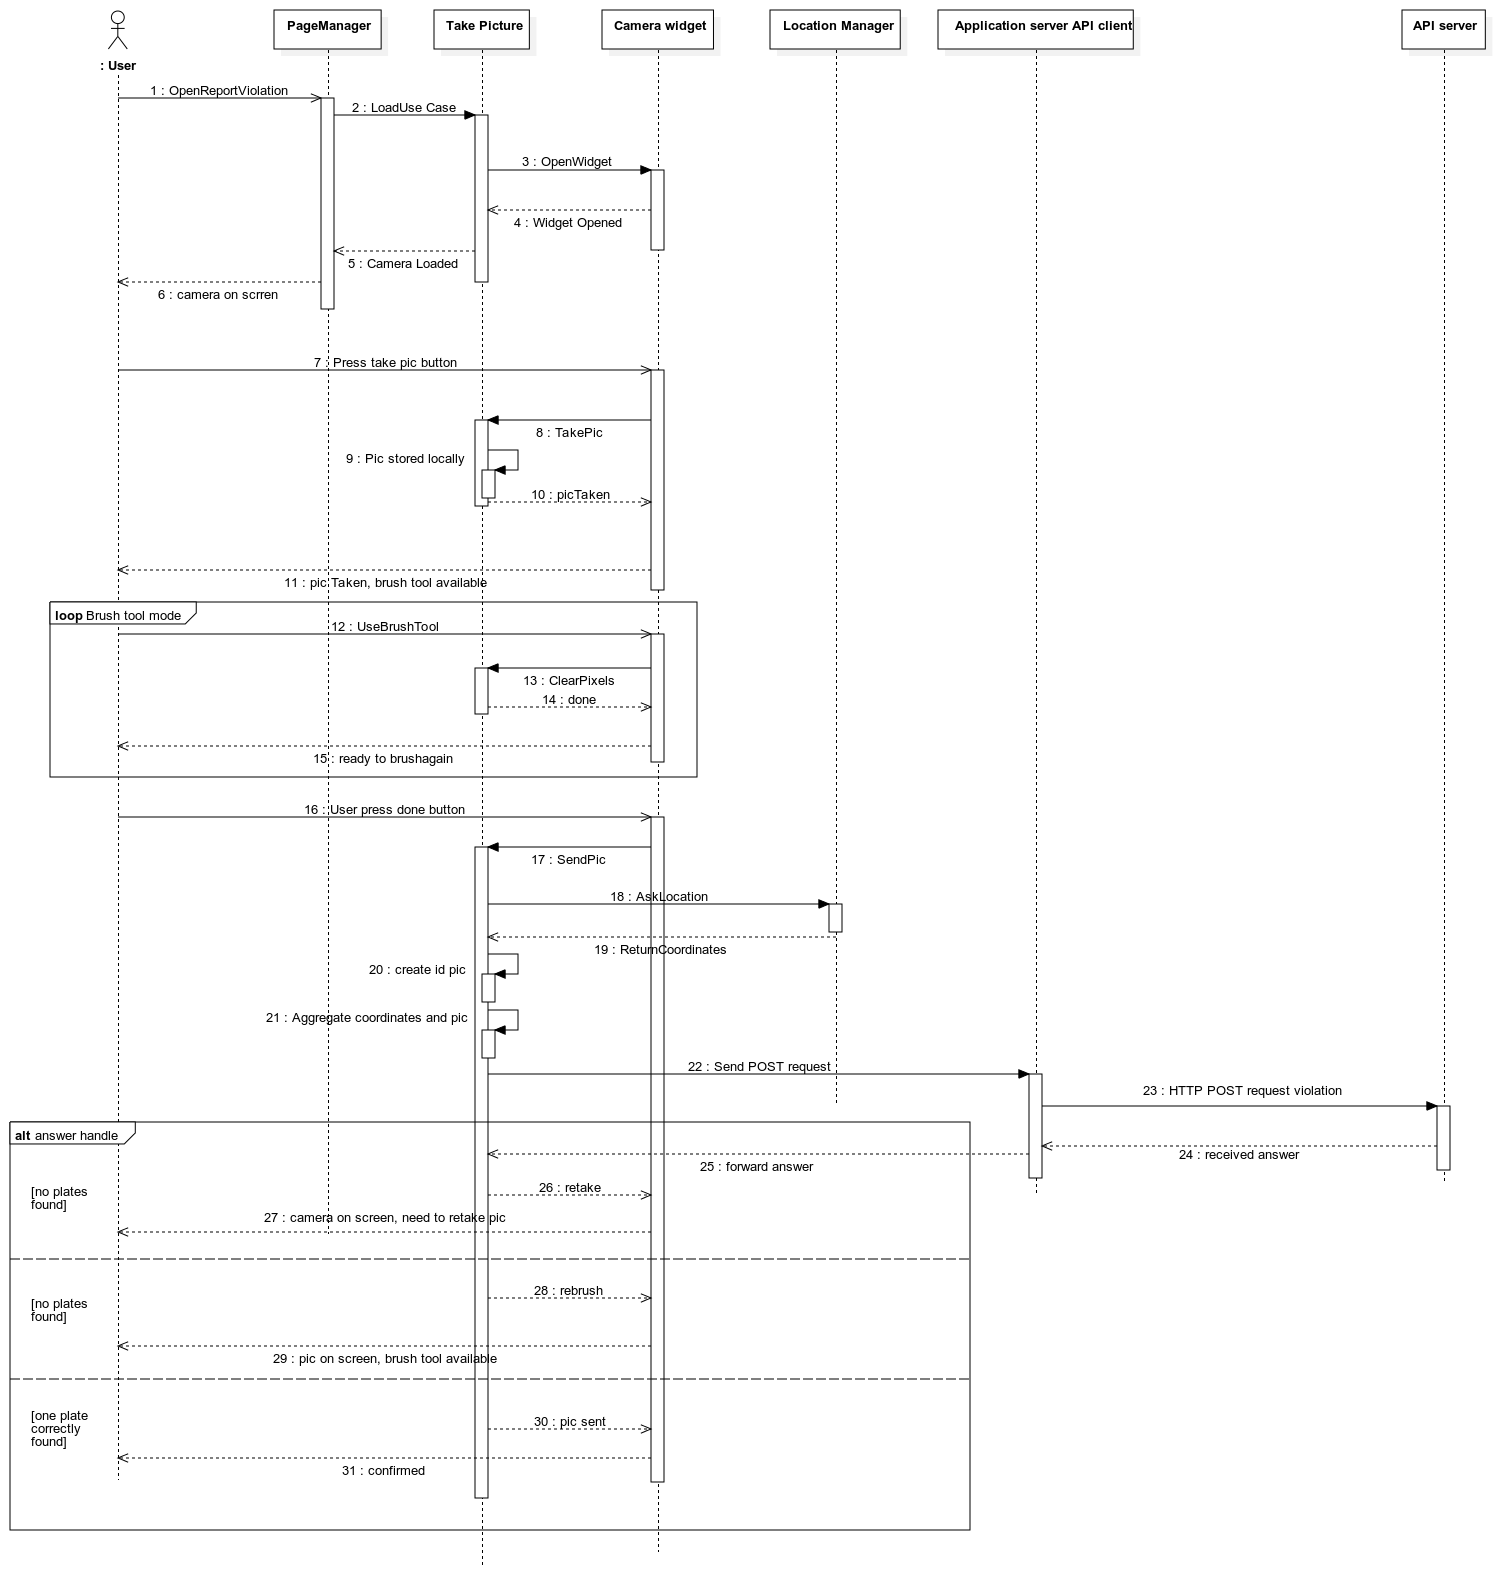
\includegraphics[width=\textwidth]{Images/DDSeqAppPic.png}
\caption{\label{fig:DDSeqAppPic} Sequence diagram for picture upload via the Mobile Application}
\end{figure}

In figure \ref{fig:DDSeqAppPic} is shown the sequence diagram for the use case of taking a picture using the mobile application.
The user interacts with the \textbf{PageManager} pressing the button to open the "Report Violation section", so the \textbf{TakePicture} use case is loaded because it's the first step needed to start the reporting of a violation. This opens the \textbf{CameraWidget} that is the component of the Presenter responible of showing on screen the camera recording. When the widget is correctly started the user can take the picture pressing the main button. The widget has to tell the \textbf{TakePicture} use case that the button has been pressed so the picture can  actually be taken and stored locally. The camera widget can now show the picture just taken and show the brush tool mode. If there is need the user can cover whith is finger some areas of the picture. The widget communicates to the use case the location of those areas so the image can be manipulated by the \textbf{TakePicture} use case and stored. This can happen until the user presses the "done button". Now the the \textbf{TakePicture} use case asks the the \textbf{LocationManager} to return the GPS coordinates of the device. An Unique identifier is generated which is passed with the picture to the \textbf{Application Server API client} which has to actually make the POST HTTP request to the Application Server (endpoint \url{/API/v1/violations/upload/id=xxx} ). What happens in the applcation server is described later in the following Sequence diagram in Figure \ref{fig:DDSeqSeverPic}.
When an answer is received there are three options possible: if no plates have been found, the use case has to start again, so it tells the widget to show a message for the user, asking to retake the picture including the plate.
If more than one plates are found, the use case has to ask the widget to show a message asking the user to use again the brush tool mode to cover the plates not required. If one plate is correctly identified the use case can tell the widget to show a success messae and terminates. %done!

\begin{figure}[H]
\centering
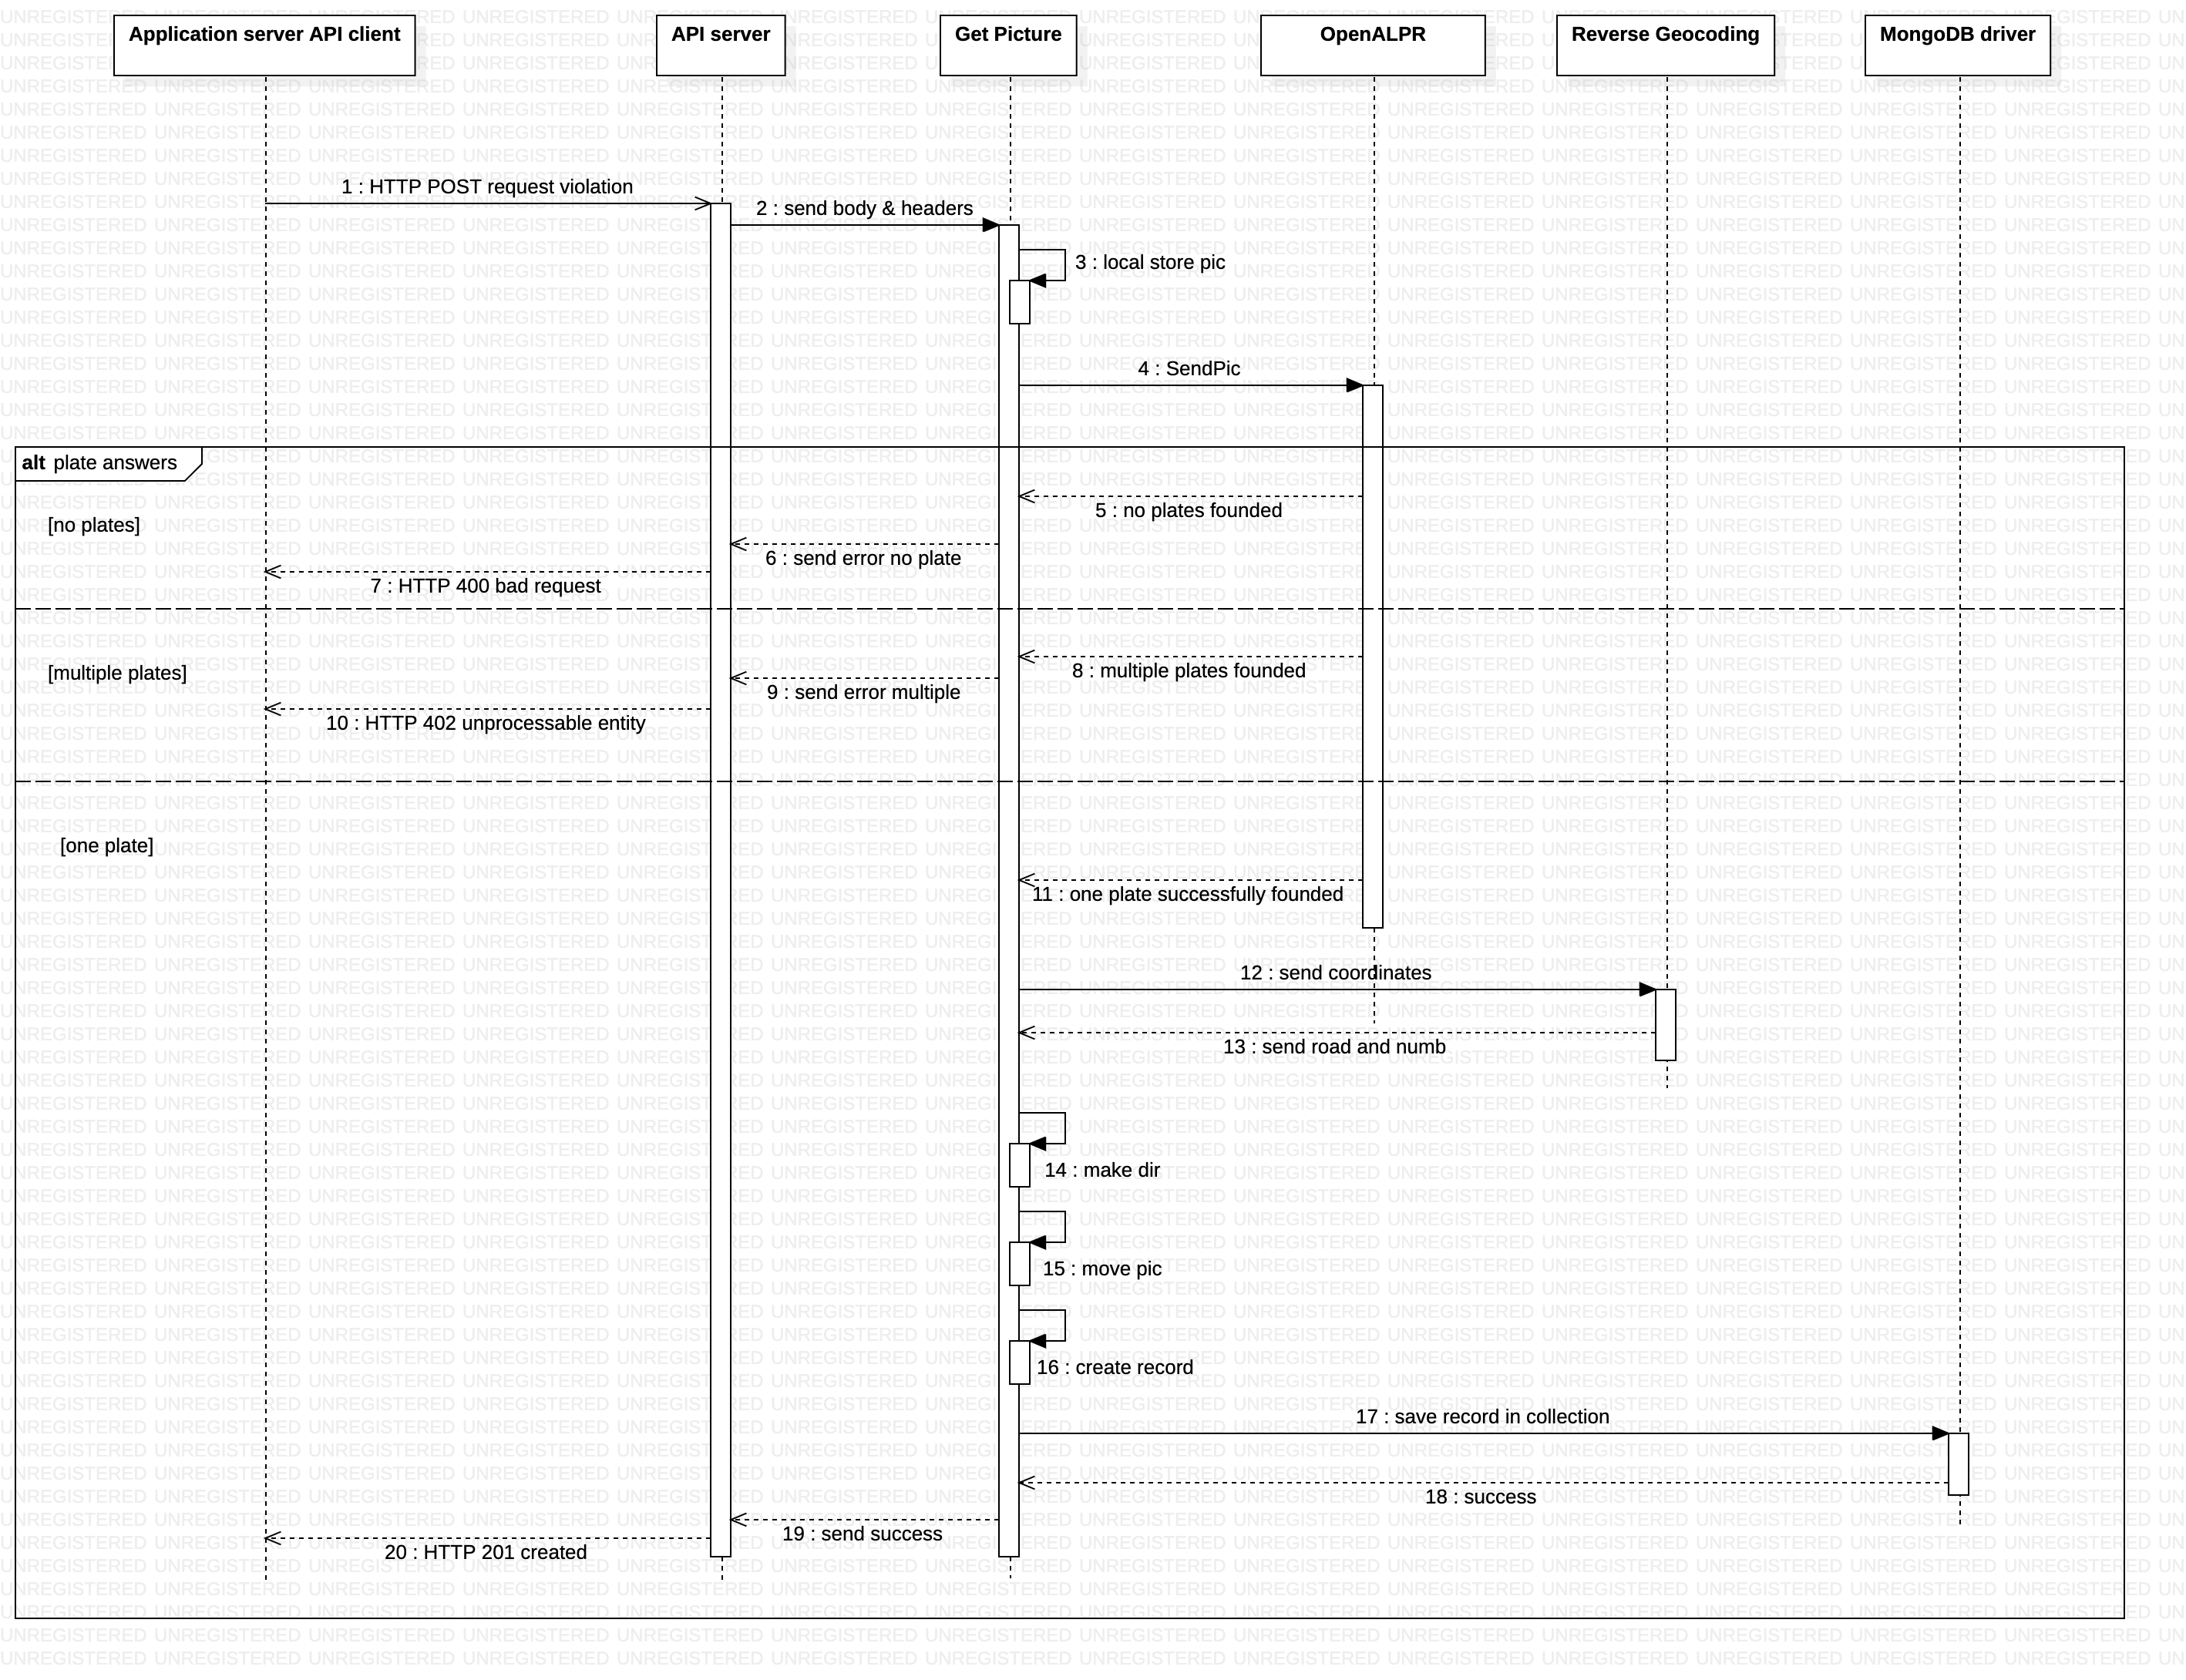
\includegraphics[width=\textwidth]{Images/DDSeqSeverPic.png}
\caption{\label{fig:DDSeqSeverPic} Sequence diagram for picture storage by Application Server}
\end{figure}
In figure \ref{fig:DDSeqSeverPic} is shown the sequence diagram for the Application Server when it receives a POST request at the endpoint \url{/API/v1/violations/upload/id=xxx} containing a new picture in the body. When the requests is receied the the picture is stored on a temporary folder of the server by the component \textbf{Get Picture}. This use case then has to call the external API \textbf{OpenALPR} sending the picture of violation in order to decode the plate number. We have three options, depeending on the answer of the call to the \textbf{OpenALPR} API.

If no plates are found, the usecase \textbf{Get Picture} has to ask the \textbf{API server} to answer to the mobile app, informing that no plates were present in the picture. One possible HTTP answer for this error is \textcolor{poliblue}{400 bad request}.

If multiple plates have been found, the usecase \textbf{Get Picture} has to ask the \textbf{API server} to answer to the mobile app, informing that more than one plate were present in the picture. One possible HTTP answer for this error is \textcolor{poliblue}{402 unprocessable entity}.

If one plate is correctly found, then there is need to get the street name and number from the coordinates received from the POST request. This is done by sending the coordiantes to the external \textbf{Reverse Geocoding} API which returns the name and the road number.
We don't store the pictures in the database, rather the use case moves the picture of the violation on a specific directory of the filesystem and then creates the document containing the path of the picture and the metadata. This is stored in the database by the \textbf{MongoDB driver}. The HTTP answer sent to the mobile app in this case is \textcolor{poliblue}{201 created}.

\begin{figure}[H]
\centering
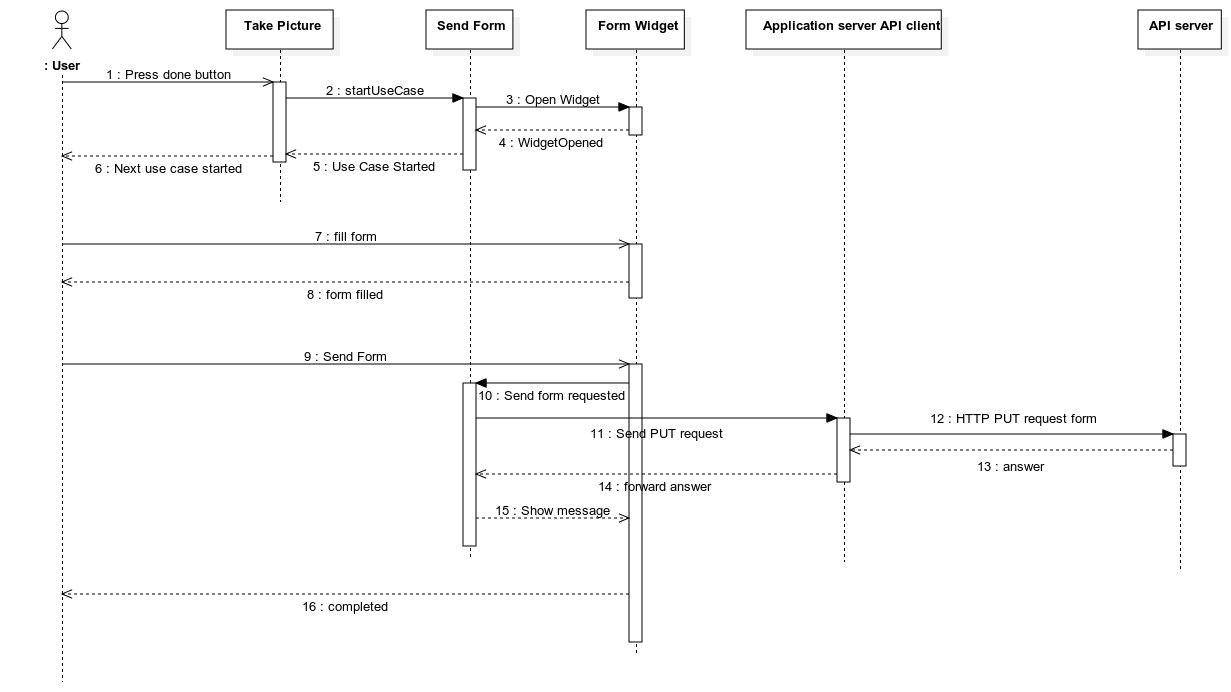
\includegraphics[width=\textwidth]{Images/DDSeqAppForm.png}
\caption{\label{fig:DDSeqAppForm} Sequence diagram for filling form on Mobile App}
\end{figure}
In figure \ref{fig:DDSeqAppForm} is shown the sequence diagram for the use case of filling the violation form in the Mobile App.
After the User has done the take and upload picture use case, the next use case \textbf{Send Form} is started. This use case requires the loading of the \textbf{Form Widget} whic shows the list of possible types of kind of violation. The user fills the form and the widget communicates to the use case the choice made. This selection then is communicated to the Application Server with a PUT request in order to update the document containing the violation document with an attribute containing the kind. This is done by the \textbf{Application server API client} using the following endpoint: \url{PUT} \url{/API/v1/violations/upload/form/id=xxx}.


\begin{figure}[H]
\centering
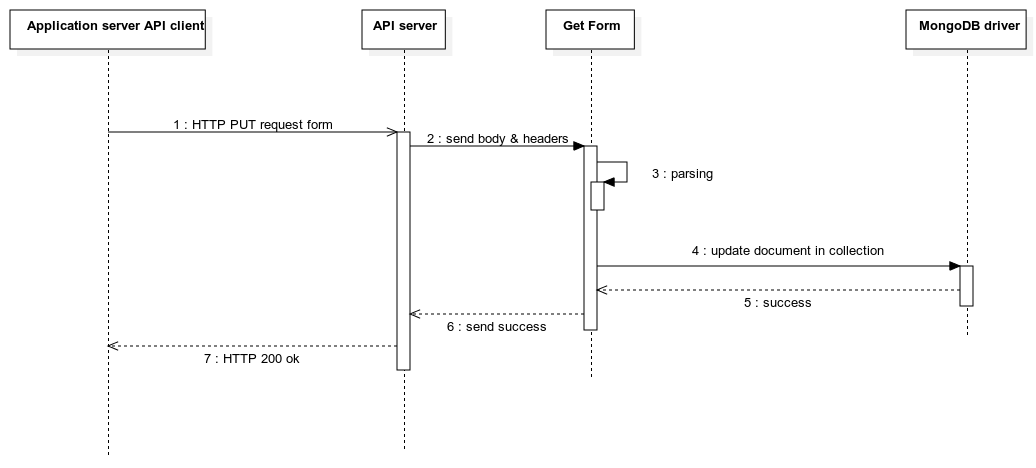
\includegraphics[width=\textwidth]{Images/DDSeqSeverForm.png}
\caption{\label{fig:DDSeqSeverForm} Sequence diagram for getting the form by Application Server}
\end{figure}

In figure \ref{fig:DDSeqSeverForm} is shown the sequence diagram for the use case of getting the content of the filled form about the kind of violation by the Application Server. When the \textbf{API server} receives a PUT request at the following URL \url{/API/v1/violations/upload/form/id=xxx} it has to forward the content to the use case \textbf{Get Form} which parses the content and updates the document stored in the databse about the violation, completing the attribute about the kind of violation. The HTTP answer sent to the mobile app after the success of this case is \textcolor{poliblue}{200}.



\subsubsection{Streets Heatmap}%%%%%%%%%%%%%%%%%%%%%%%%%%%%%%%%%%%%%%%%%%%%%%%%%%%%%%%
\begin{figure}[H]
\centering
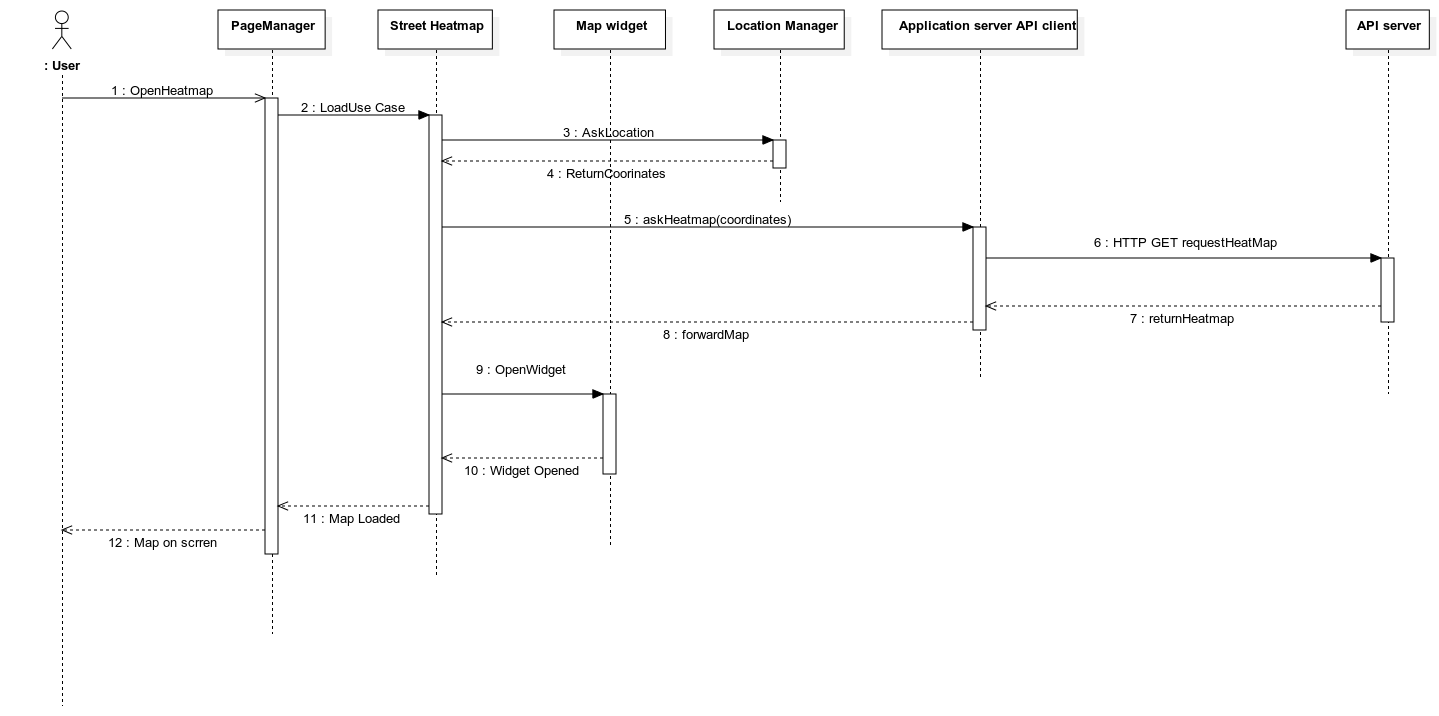
\includegraphics[width=\textwidth]{Images/DDSeqAppMap.png}
\caption{\label{fig:DDSeqAppMap} Sequence diagram for showing Heatmap on Mobile App}
\end{figure}

In Figure \ref{fig:DDSeqAppMap} is shown the sequence diagram for the use case of showing the Heatmap of violations.
The user interacts with the \textbf{PageManager} asking to open the section with the Heatmap, with the result that the use case \textbf{Street Heatmap} is loaded. This use case first has to use the internal component interface with the controller in order to know the location of the user. This is done by calling the \textbf{Location Manager}. Then it has to interact with the API in order to retrieve the actual map with the following request: \url{GET} \url{/API/v1/heatmap/lat=xxx&long=xxx}.
Once the map is returned the \textbf{Map Widget} can be opened.

\begin{figure}[H]
\centering
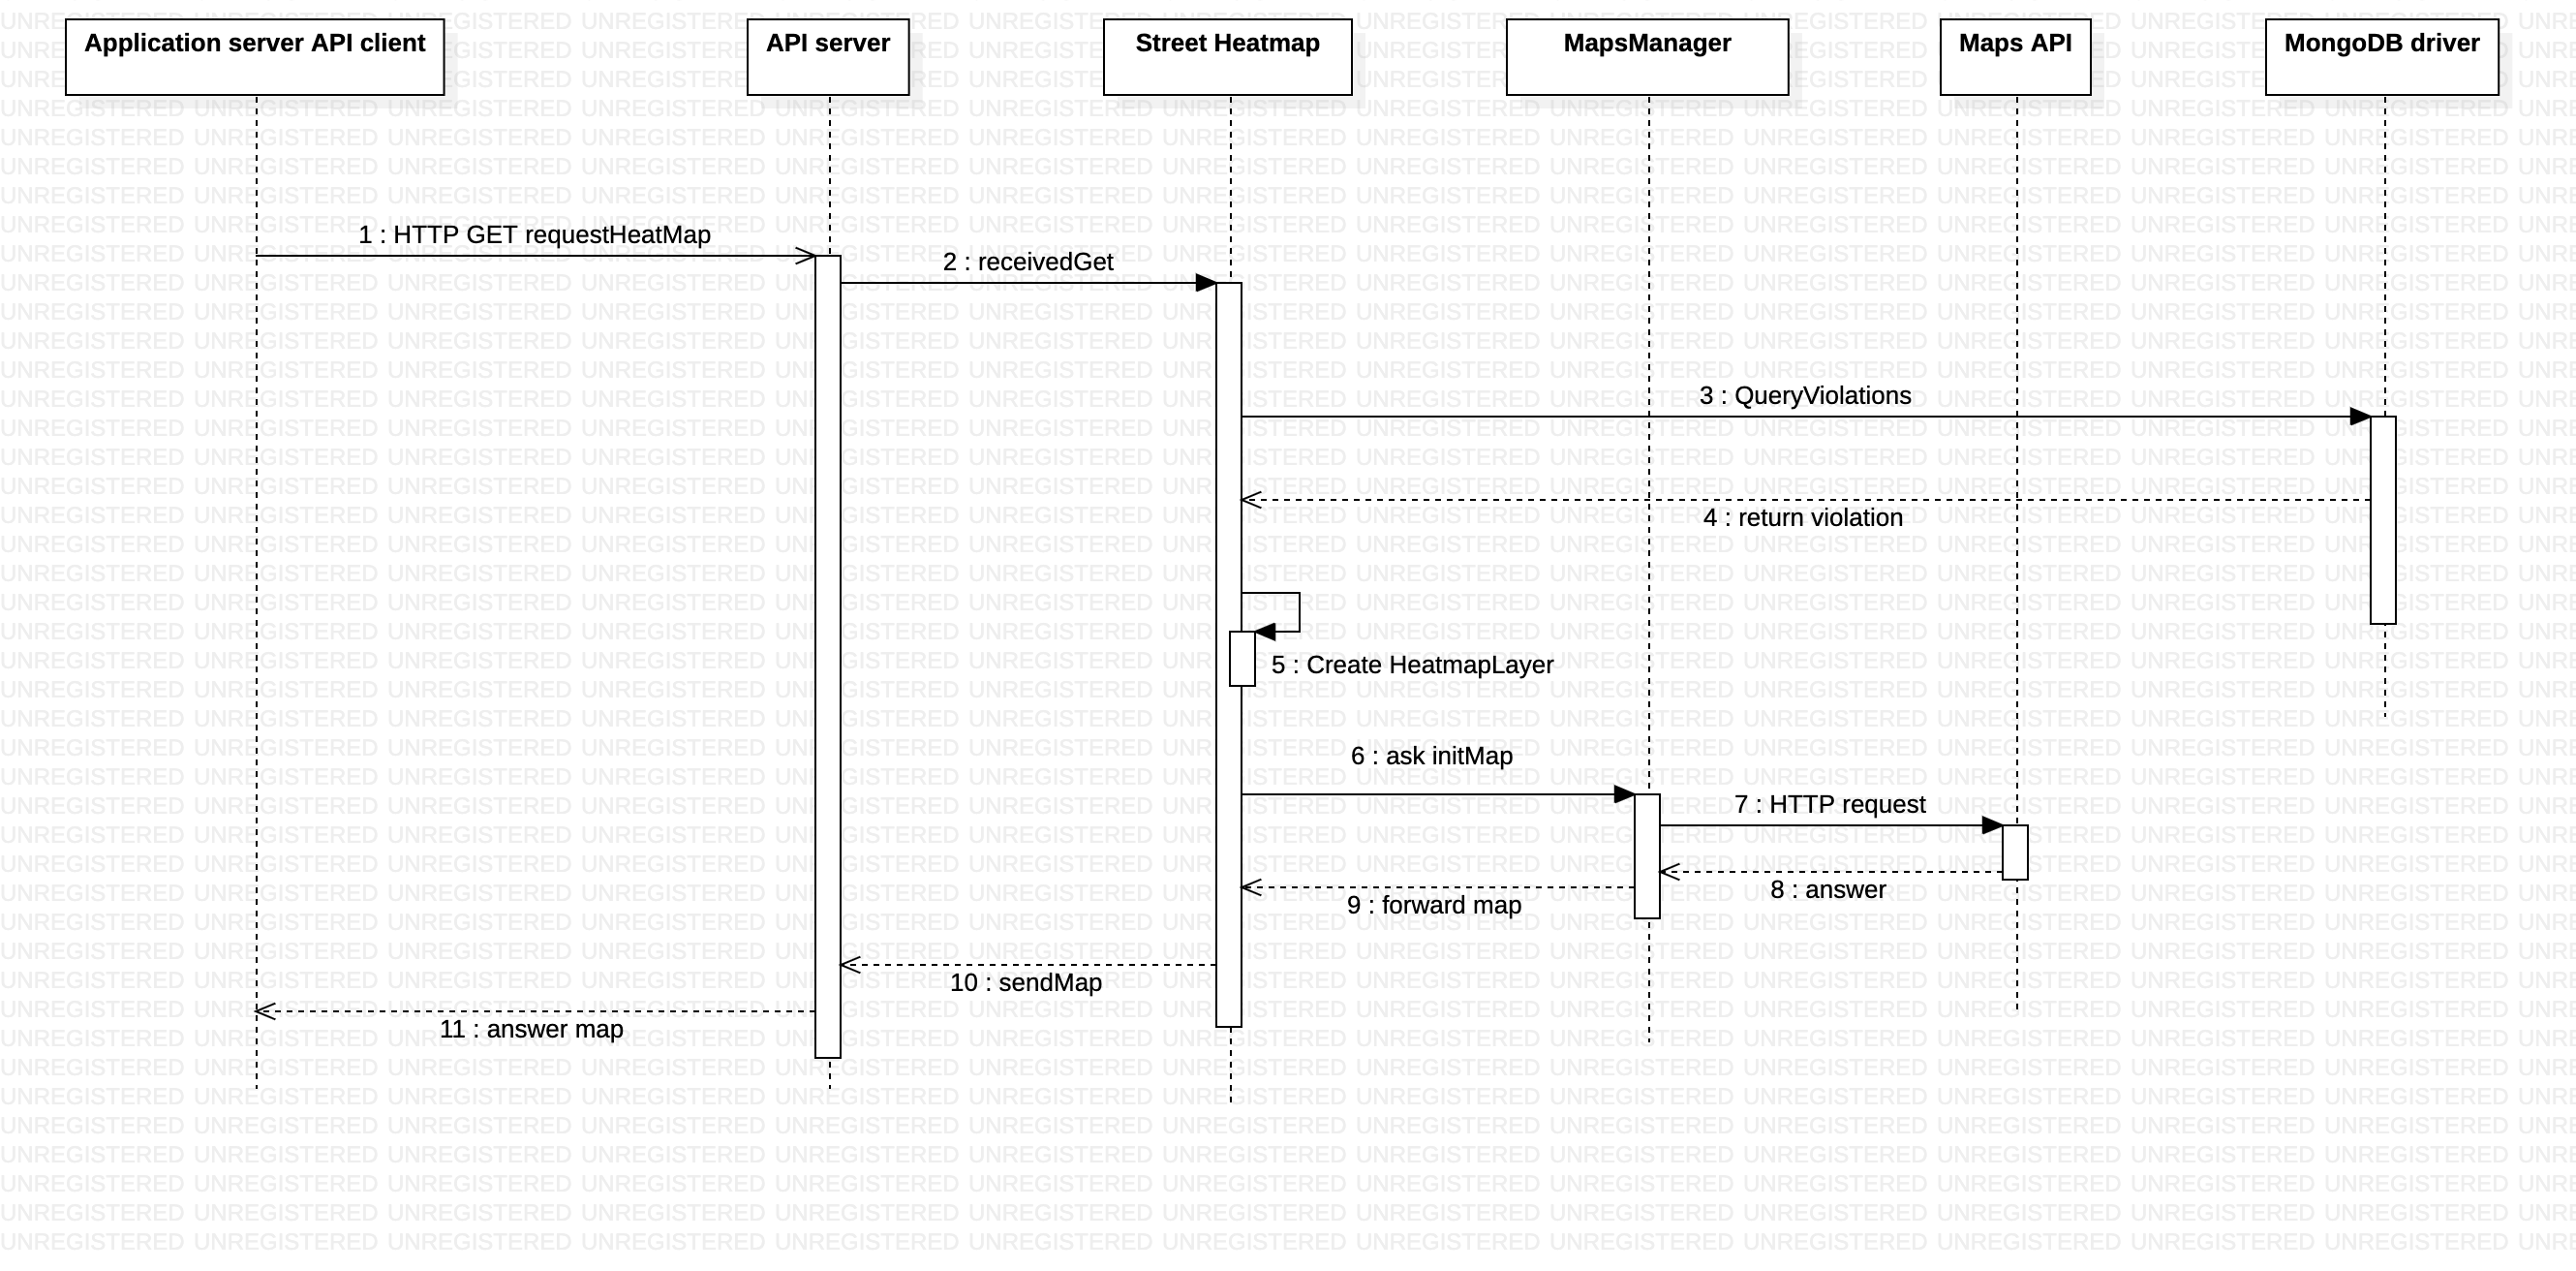
\includegraphics[width=\textwidth]{Images/DDSeqSeverMap.png}
\caption{\label{fig:DDSeqSeverMap} Sequence diagram for creating Heatmap on Application Server}
\end{figure}

In figure \ref{fig:DDSeqSeverMap} is shown the sequence diagram for the use case of creating the Heatmap on the Application Server.
Once the server receives a GET request from the endpoint devoted offer the Heatmap (example: \url{/API/v1/heatmap/lat=xxx&long=xxx}) the first thing that it does is querying the database containing all the violations, getting the coordiantes of each violation reported. The Heatmap Layer is part of the \textcolor{poliblue}{google.maps.visualization} library, which must be loaded. Using the data from violations it's now possible to create a \textcolor{poliblue}{HeatmapLayer} object containing the latitude and longitude of every violation that must be visualized \cite{GMapsHeat}. After instantiating the \textcolor{poliblue}{HeatmapLayer} object it has to be added to the map by calling the \textcolor{poliblue}{setMap()} method of the Google Maps API \cite{GMapsHeat}. All the data of the map must be than forwarded to who made the GET request.
Using this logic we are in fact "mirroring" the Google Maps API on our Application Server. This approach has the following advantage: the mobile APP has only to interact with our Application Server which manages all the map creation (using the external service). So on the mobile app there is no nead to add a dedicated controller for the Maps service.

\subsubsection{Vehicle list by violations}%%%%%%%%%%%%%%%%%%%%%%%%%%%%%%%%%%%%%%%%%%%%%%%%%%%%%%%
\begin{figure}[H]
\centering
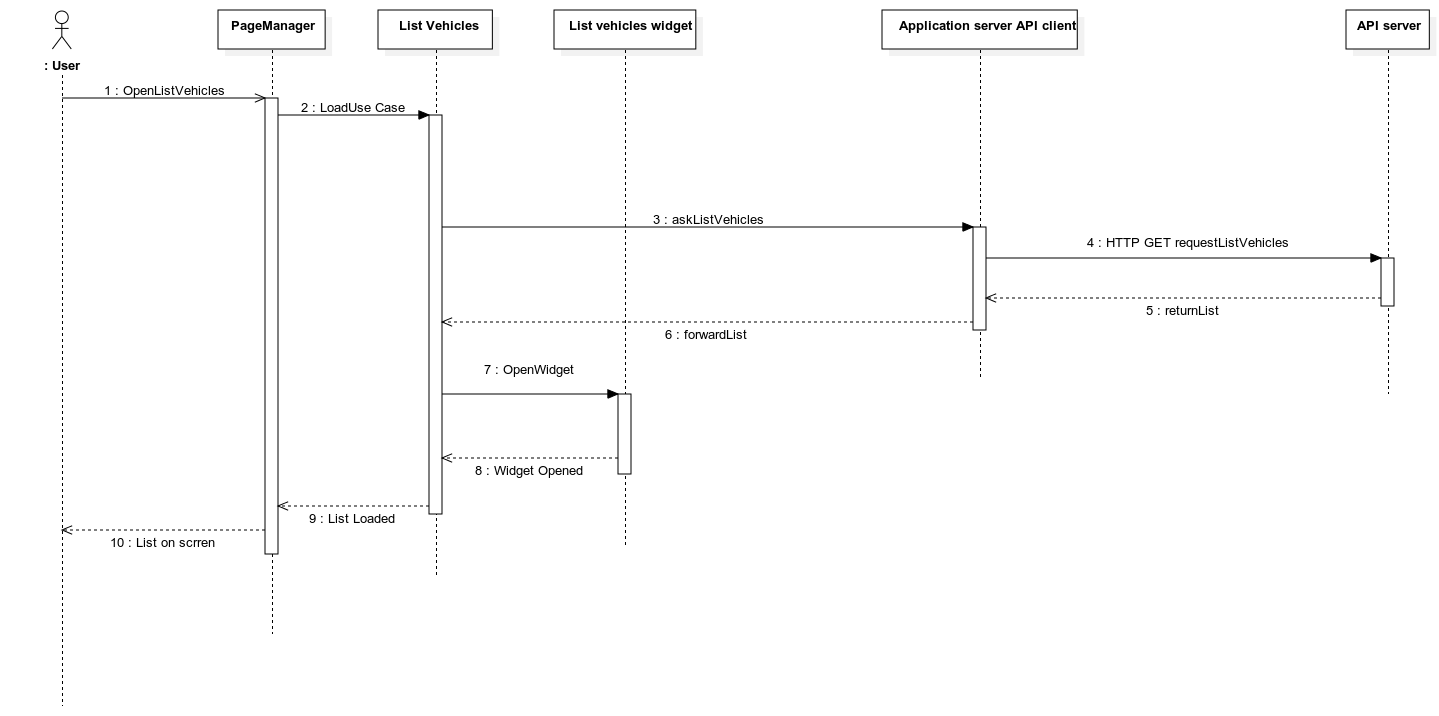
\includegraphics[width=\textwidth]{Images/DDSeqAppList.png}
\caption{\label{fig:DDSeqAppList} Sequence diagram for showing list of vehicles ordered by violations in Mobile App }
\end{figure}

In Figure \ref{fig:DDSeqAppList} is shown the sequence diagram for the use case of showing the list of plates ordered by number of violations.
The user interacts with the \textbf{PageManager} asking to open the section with the list of violators, with the result that the use case \textbf{List Vehicles} is loaded. This use case has to interact with the API in order to retrieve the list of vehicles associated with the count of violations. This is dove with a GET request that must also specify the number of records than needed to be retreived. As for example: \url{GET} \url{/API/v1/violations/plates.json?countby=violations&sort=desc&depth=x}. So the use case calls the \textbf{Application server API client}  which performs the actual call to the REST API. Once a JSON file containing the data required is returned by the API, the use case can open the \textbf{List vehicles widget} responsible of showing on the app the list.


\begin{figure}[H]
\centering
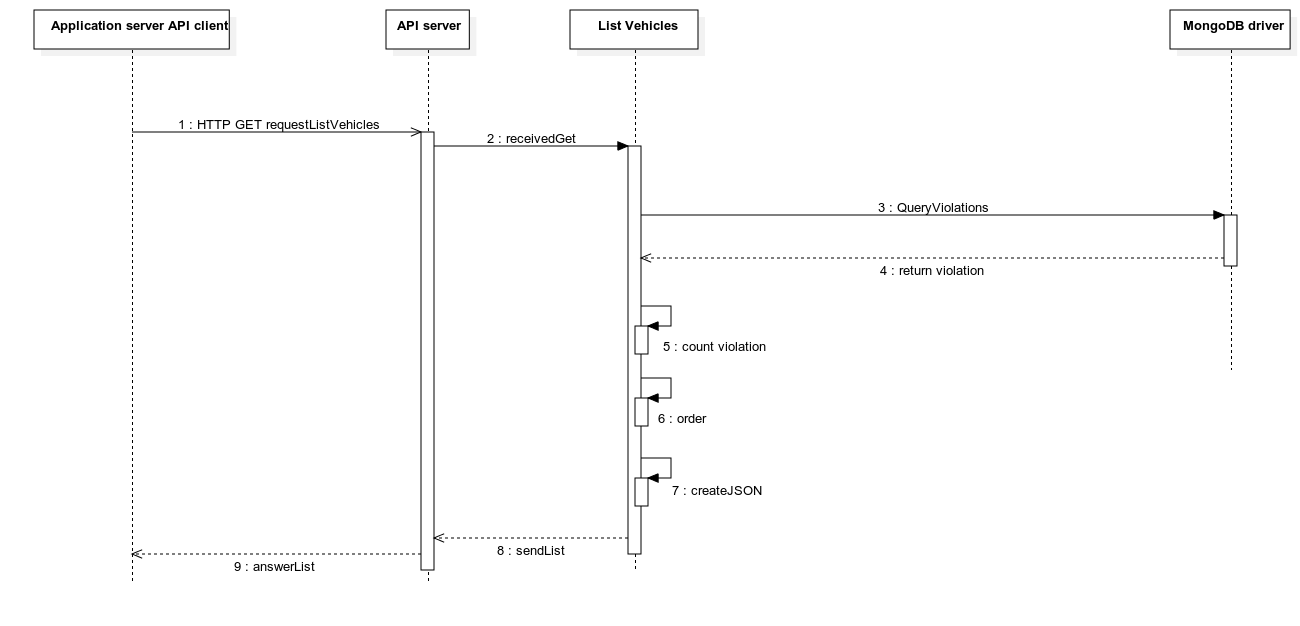
\includegraphics[width=\textwidth]{Images/DDSeqSeverList.png}
\caption{\label{fig:DDSeqSeverList} Sequence diagram for getting list of vehicles ordered by violations in Application Server  }
\end{figure}
In Figure \ref{fig:DDSeqSeverList} is shown the sequence diagram for the use case of getting from database the list of vehicles that committed the most violations, ordering and then offering the API endpoint.
Once the server receives a GET request from the endpoint devoted to the list of violations (example: \url{/API/v1/violations/plates.json?countby=violations&sort=desc&depth=x}) it has to query the database of violations and count the number of violation for each unique plate. Then it must sort them in descending order and creating a JSON file that must be returned to who called the API. The numner of record returned was specified in the GET request.


\subsubsection{Ticket Creation}%%%%%%%%%%%%%%%%%%%%%%%%%%%%%%%%%%%%%%%%%%%%%%%%%%%%%%%
\begin{figure}[H]
\centering
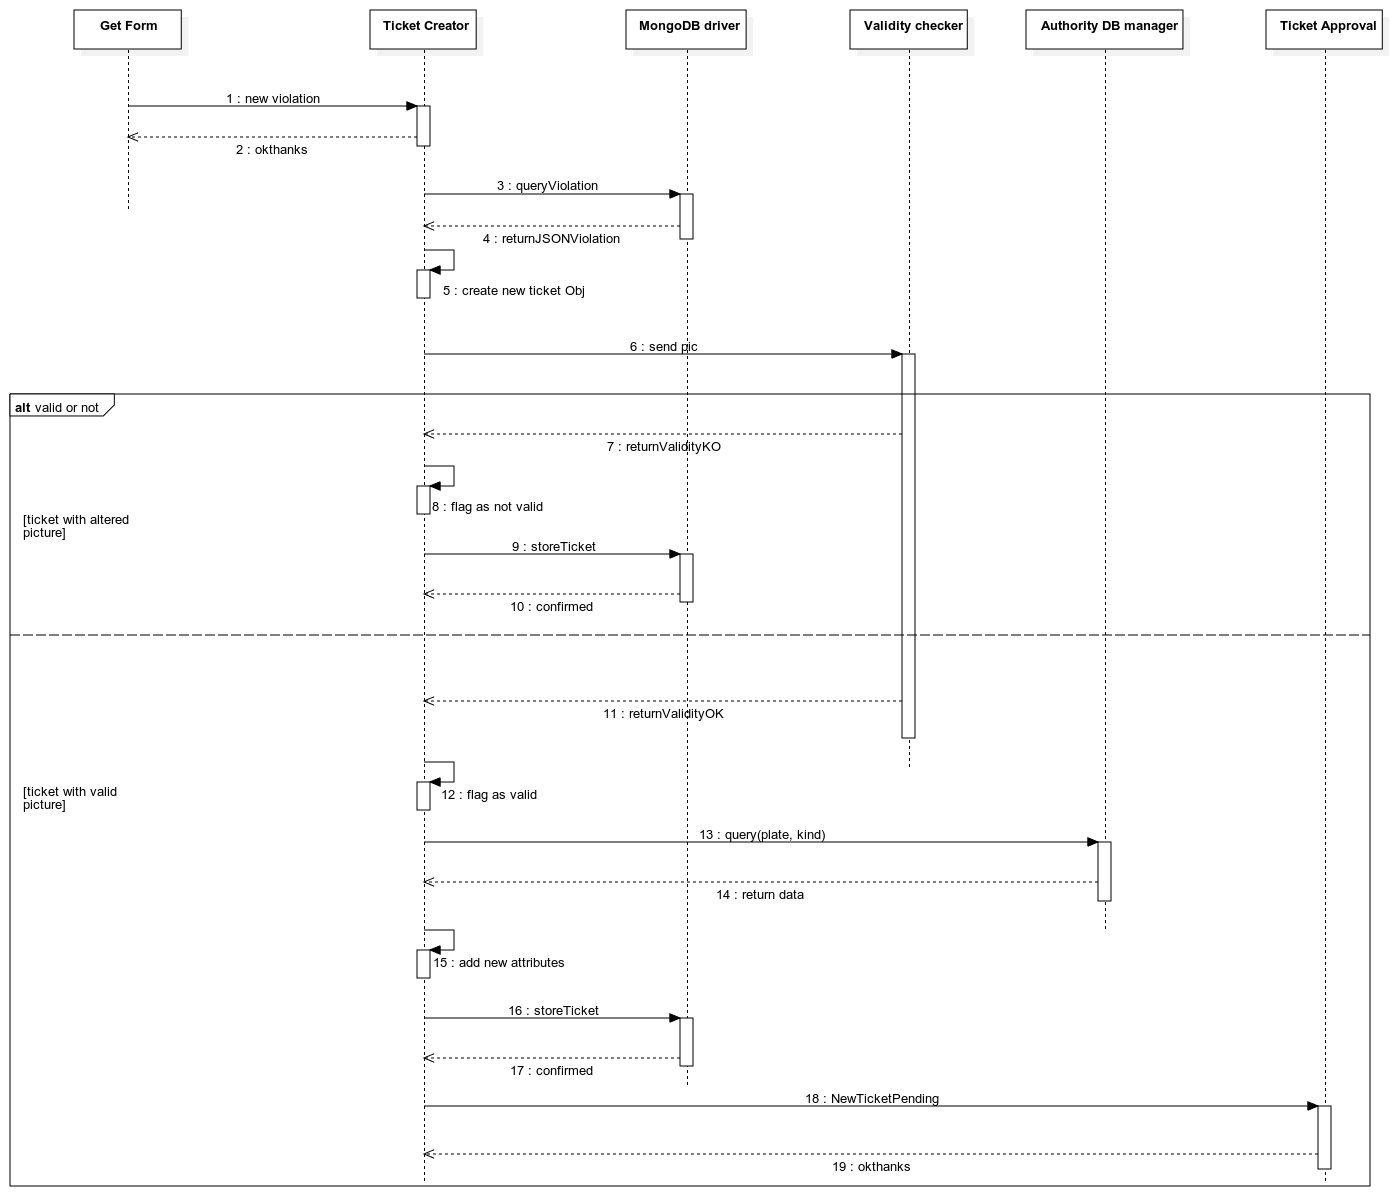
\includegraphics[width=\textwidth]{Images/DDSeqSeverTickCreat.png}
\caption{\label{fig:DDSeqSeverTickCreat}} Sequence diagram for ticket Creation in Application Server
\end{figure}

In Figure \ref{fig:DDSeqSeverTickCreat} is shown the sequence diagram for the use case of creating a ticket from an inserted violation in the Application Server.
When a new violation has been successfully inserted, the use case \textbf{Get Form}, sends a message to the use case \textbf{Ticket Creator} informing that a new violation is available in the database so it's possible to start creating the corresponding ticket. Now the \textbf{Ticket Creator} knows the ID of the new inserted violation so it can query the Database for that specific violation. Then it uses the queried data of the violation to create a new Ticket Object. To check if the picture of the violation hasn't been altered it passes to the component \textbf{Validity checker} the path of the picture so it can be sent to the external service. Once the answer is received, we have to alternetives. If the picture is considered fake, the ticket attribute \textcolor{poliblue}{valid} is set to FALSE and the ticket is stored in the database for debu purposes or for cheater identification which can be later implemented.
If the picture was authentic the ticket attribute \textcolor{poliblue}{valid} is set to TRUE. Then there is need to complete some attributes of the ticket quering the external Authority database. This is done by calling the component \textbf{Authority DB manager}. These attributes are: the name, surname and address of the owner of the violator, the amount of money to be paid and the deadline of payment for that kid of violation. After the new attributes are added to the Ticket object, it is stored in the database. Lastly a message to the use case \textbf{Ticket Approval} is sent, telling the ID of the new isnerted ticket.
%%done!

\subsubsection{Ticket Approval}%%%%%%%%%%%%%%%%%%%%%%%%%%%%%%%%%%%%%%%%%%%%%%%%%%%%%%%
\begin{figure}[H]
\centering
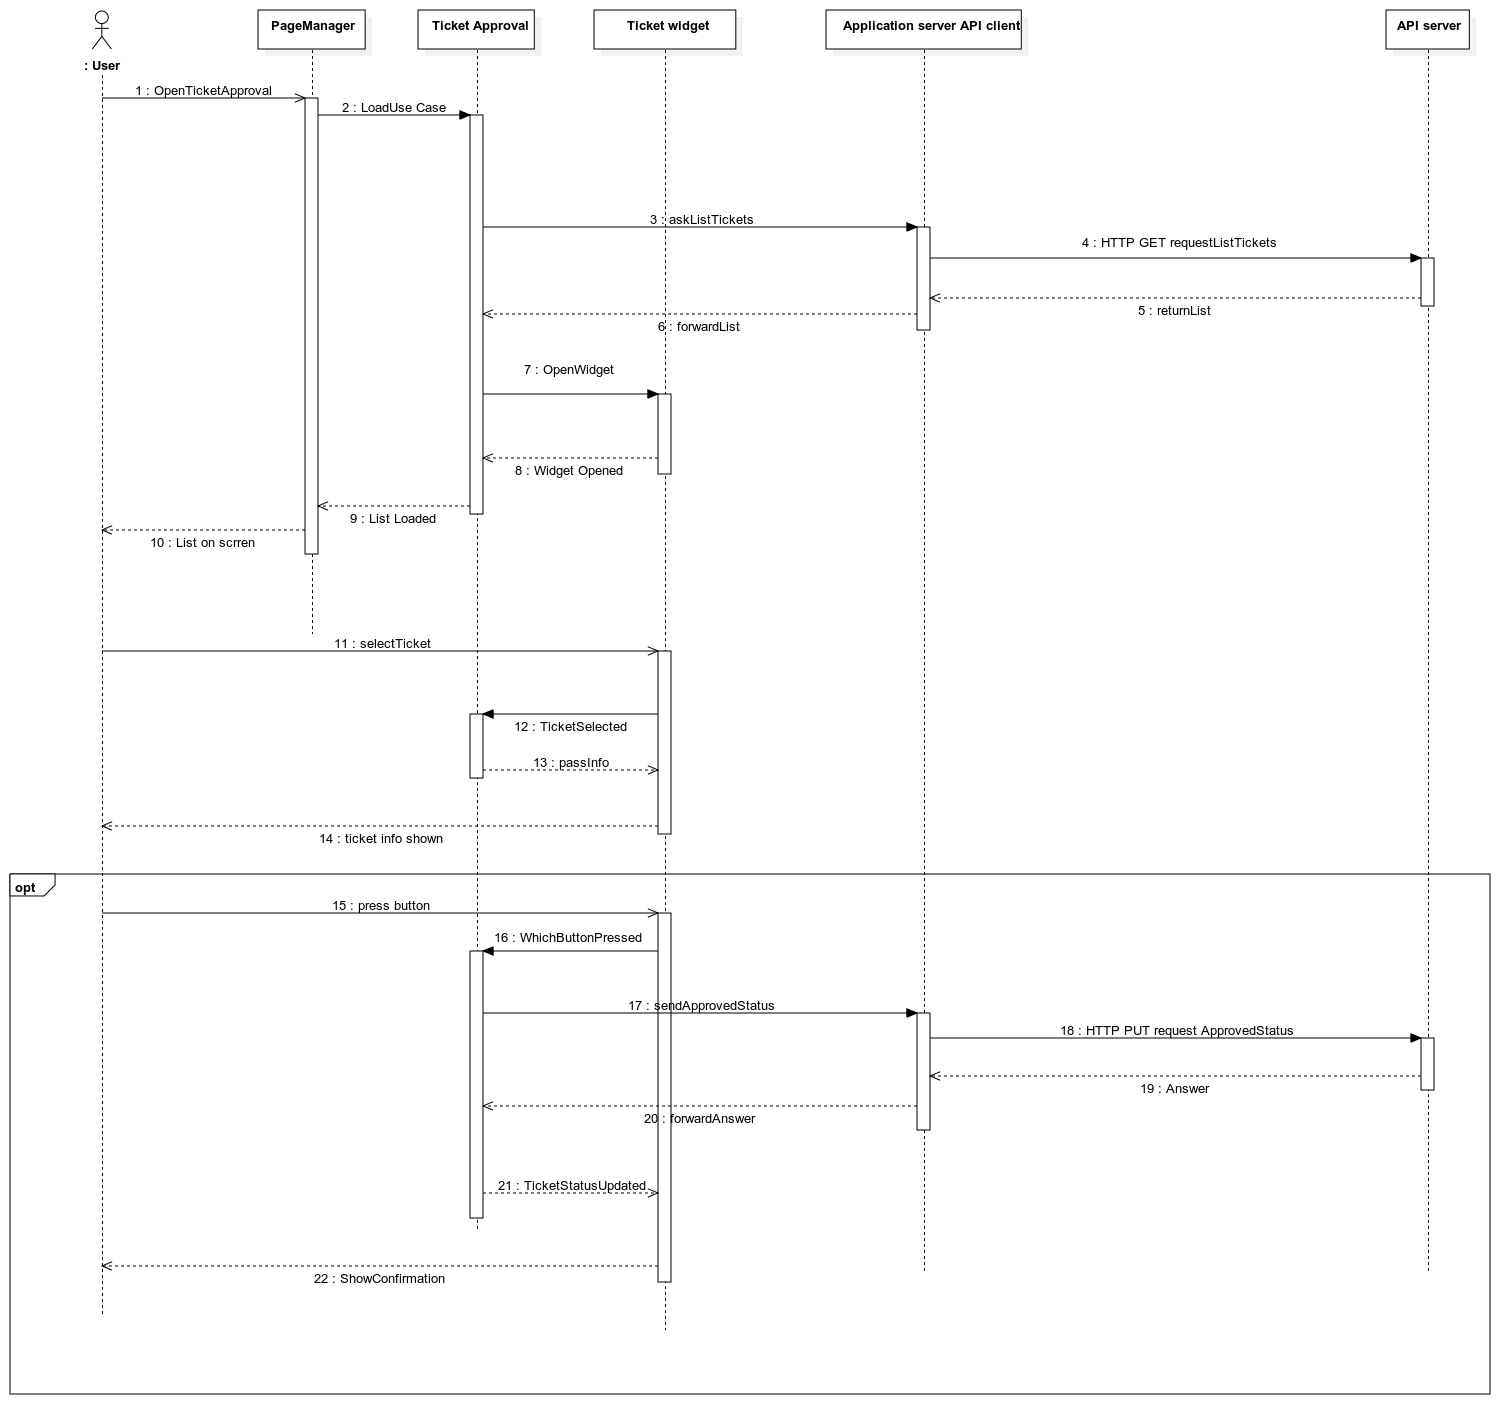
\includegraphics[width=\textwidth]{Images/DDSeqAppTick.png}
\caption{\label{fig:DDSeqAppTick}} Sequence diagram for Ticket Approval on the Mobile Application
\end{figure}
In Figure \ref{fig:DDSeqAppTick} is shown the sequence diagram for the use case of approving a ticket on the mobile Application.
The user interacts with the \textbf{PageManager} asking to open the section of ticket approval, with the result that the use case \textbf{Ticket Approval} is loaded. The \textbf{PageManager} only offers this function to the authority users, as stated in the RASD, this is a function only for policemen. This use case has to interact with the API in order to retrieve the list of pending tickets. This is dove with a GET request. As for example: \url{GET} \url{/API/v1/tickets/pending.json}. So the use case calls the \textbf{Application server API client} which performs the actual call to the REST API. Once a JSON file containing the data required is returned by the API, the use case can open the \textbf{Ticket widget} responsible of showing on the app the list.
If the user selects a ticket, the widget sends a message to the use case with the ID of the ticket and receives back the information relative to that one. So the deatil of the ticket is shown on screen with a button for approval or discarding. When one of those buttons is pressed, the \textbf{Ticket widget} communicates to the use case which selection has been made by the user. This selection then is communicated to the Application Server with a PUT request in order to update the document containing the ticket with an attribute to determine if has been approved or not. The choice made is sent in the body of the following request: \url{PUT} \url{/API/v1/tickets/ticketid}
